\documentclass[12pt]{article}
\usepackage[utf8]{inputenc}

\usepackage[a4paper, margin=1in]{geometry}
\usepackage{newtxtext}
\usepackage{amsmath,amssymb,amsthm}
\usepackage{newtxmath} % must come after amsXXX

\usepackage{float} % to prevent figure floating

\usepackage{graphicx}

\usepackage{tabularx} % Include this in the preamble

%\usepackage{subfigure}

\usepackage{xcolor}
\usepackage{fancyhdr}
\usepackage{listings}
%\usepackage{ctex}
\usepackage{booktabs}

%%%%%%%%%%%% for pseudocode %%%%%%%
\usepackage{algorithm}
\usepackage{algorithmic}
\usepackage{algpseudocode}
%%%%%%%%%%%%%%%%%%%%%%%%%%%%%%%%%%

\usepackage{array}  % For wrapping text in columns
\usepackage{lipsum} % For placeholder text (optional)


\makeatletter
\renewcommand\paragraph{\@startsection{paragraph}{4}{\z@}%
% display heading, like subsubsection
                                     {-3.25ex\@plus -1ex \@minus -.2ex}%
                                     {1.5ex \@plus .2ex}%
                                     {\normalfont\normalsize\bfseries}}
 \setcounter{secnumdepth}{4}
\makeatother

\usepackage{amsmath,amsfonts,amssymb}
\usepackage{geometry}
\usepackage{graphicx}
\usepackage{caption}
\usepackage{fancyhdr}
\usepackage{titling}
\usepackage{lipsum}  % This package provides filler text, remove it in your actual document

\usepackage{overpic} % put table on the figure

\geometry{
 a4paper,
 total={170mm,257mm},
 left=20mm,
 top=20mm,
}

% Header and Footer settings
\pagestyle{fancy}
\fancyhf{}
\cfoot{\thepage}
\renewcommand{\headrulewidth}{0pt}
\renewcommand{\footrulewidth}{0pt}

\title{Falling Drop Simulation--Reapproach}
\author{Haobo Zhao}
\date{\today}

\begin{document}

\maketitle


\begin{abstract}
This study presents numerical simulations of a falling liquid drop through another fluid using the Front Tracking method to accurately capture interface dynamics. The incompressible Navier-Stokes equations are solved, and characteristic parameters were set up to investigate the effects of varying Eötvös numbers ($Eo$) and Ohnesorge numbers ($Oh$) on the drop's deformation, velocity, and breakup behavior. A grid independence study ensures the accuracy of the results. Simulations reveal that higher $Eo$ leads to increased deformation and earlier breakup. Comparisons with existing literature validate the model, we now have better understanding of the falling drop behaviour and the effect of domain non-dimensional numbers and the forces behind them.
\end{abstract}



\section{Introduction}

The behavior of a falling drop through another fluid is a fundamental problem in fluid dynamics with wide-ranging applications. Understanding this phenomenon is crucial for processes such as rainfall formation, inkjet printing, spray cooling, and fuel injection systems. In these contexts, the dynamics of drop deformation, oscillation, and breakup directly affect efficiency and performance.

For instance, in environmental science, the breakup of raindrops influences weather patterns and soil erosion. In industrial applications, controlling droplet behavior is essential for optimizing combustion in engines, improving coating technologies, and enhancing drug delivery in aerosols. Studying the transient evolution of a falling drop provides valuable insights that can be applied to design and optimize systems involving multiphase flows.

% \subsection{Research Overview of Falling Drop Along time}
\begin{table}[htbp]
\scriptsize
\centering
\caption{Key Studies and Approaches on Drop Dynamics (Part 1)}
\renewcommand{\arraystretch}{1.2} % Adjust row height for better spacing
\begin{tabularx}{\textwidth}{|c|X|X|}
\hline
\textbf{Ref} & \textbf{Key Approach} & \textbf{Result/Contribution} \\ \hline
Stokes, 1851 \cite{stokes1851pendulums} & Analytic solution for viscous drag on small spheres & Established Stokes' law, applicable to small falling droplets \\ \hline
Worthington, 1876 \cite{worthington1876study} & First experimental capture of falling drop dynamics & Laid the experimental foundation for drop dynamics studies \\ \hline
Rayleigh, 1878 \cite{rayleigh1878instability} & Stability of liquid jets & Foundation for instability phenomena in fluid dynamics \\ \hline
Taylor, 1934 \cite{taylor1934emulsions} & Study of emulsion formation in flow fields & Key insights into the relationship between surface tension and flow \\ \hline
Proudman \& Pearson, 1957 \cite{proudman1957expansion} & Expansion at small Reynolds number & Showed shape deformation and velocity relationship for falling droplets \\ \hline
Hirt \& Nichols, 1981 \cite{hirt1981volume} & Volume of Fluid (VOF) method for free boundary dynamics & Developed a widely-used numerical method for multiphase flow simulations \\ \hline
Brackbill et al., 1992 \cite{brackbill1992continuum} & Surface tension models in numerical methods & Introduced surface tension models into methods like VOF \\ \hline
\end{tabularx}
\end{table}

\begin{table}[htbp]
\scriptsize
\centering
\caption{Key Studies and Approaches on Drop Dynamics (Part 2)}
\renewcommand{\arraystretch}{1.2} % Adjust row height for better spacing
\begin{tabularx}{\textwidth}{|c|X|X|}
\hline
\textbf{Ref} & \textbf{Key Approach} & \textbf{Result/Contribution} \\ \hline
Peregrine et al., 1997 \cite{peregrine1997impact} & Investigation of drop impact on liquid surfaces & Studied splashing phenomena during droplet impacts \\ \hline
Eggers, 1997 \cite{eggers1997nonlinear} & Nonlinear dynamics and breakup of free-surface flows & Described the nonlinearity and singularities in droplet splitting \\ \hline
Han \& Tryggvason, 1999 \cite{han1999axisymmetric} & Axisymmetric drop breakup using CFD & Studied drop breakup with parameters like Eo, Oh, Re, and We \\ \hline
Brenner et al., 1999 \cite{brenner1999breakup} & Study of viscous liquid breakup & Provided detailed analysis of droplet breakup mechanisms \\ \hline
Thoroddsen et al., 2008 \cite{thoroddsen2008highspeed} & High-speed photography of droplet impacts & Captured droplet collision and fragmentation at extreme velocities \\ \hline
Popinet, 2009 \cite{popinet2009accurate} & Accurate adaptive solver for interfacial flows & Developed Gerris, an open-source tool for high-precision simulation of droplet dynamics \\ \hline
Prosperetti, 2015 \cite{prosperetti2015life} & Numerical simulations of fluid-fluid interactions with high accuracy & Improved accuracy in the simulation of fluid-fluid interaction phenomena \\ \hline
Fuster \& Popinet, 2018 \cite{fuster2018allmach} & All-Mach method for bubble dynamics and surface tension simulations & Provided simulations of complex two-phase flows with high-performance computing \\ \hline
\end{tabularx}
\end{table}



\section{Solution Approach}

\subsection{Mathematical Formulation}

The motion of a falling drop is governed by the incompressible Navier-Stokes equations:

\begin{equation}
    \nabla \cdot \mathbf{u} = 0, \quad
    \rho \left( \frac{\partial \mathbf{u}}{\partial t} + \mathbf{u} \cdot \nabla \mathbf{u} \right ) = -\nabla p + \nabla \cdot \left[ \mu \left( \nabla \mathbf{u} + (\nabla \mathbf{u})^\mathrm{T} \right) \right] + \rho \mathbf{g} + \mathbf{F}_\sigma,
    \label{eq:navier_stokes}
\end{equation}

where $\mathbf{u}$ is velocity, $p$ is pressure, $\rho$ is density, $\mu$ is viscosity, $\mathbf{g}$ is gravity, and $\mathbf{F}_\sigma$ is the surface tension force modeled as $\mathbf{F}_\sigma = \sigma \kappa \delta_s \mathbf{n}$ \cite{brackbill1992continuum}, with $\sigma$ surface tension coefficient, $\kappa$ interface curvature, $\delta_s$ Dirac delta function at the interface, and $\mathbf{n}$ unit normal vector.

We employ the Front Tracking method \cite{tryggvason2011multiphase} to capture the interface, representing it with marker points $\mathbf{x}_f$ moving with the fluid velocity:

\begin{equation}
    \frac{d \mathbf{x}_f}{d t} = \mathbf{u}(\mathbf{x}_f).
    \label{eq:front_tracking}
\end{equation}

\subsection{Numerical Method}

The equations are discretized using finite differences on a staggered grid; time integration employs a second-order Runge-Kutta scheme. The pressure-Poisson equation, derived from the continuity equation, is solved iteratively to enforce incompressibility.

The computational steps are:

\begin{enumerate}
    \item Initialize $\mathbf{u}$, $p$, $\rho$, $\mu$, and interface markers $\mathbf{x}_f$.
    \item For each time step:
    \begin{enumerate}
        \item Update interface markers using Eq.~(\ref{eq:front_tracking}).
        \item Update $\rho$, $\mu$ based on the interface position.
        \item Compute $\mathbf{F}_\sigma$ and distribute it onto the grid.
        \item Compute intermediate velocity $\mathbf{u}^*$ without pressure.
        \item Solve the pressure-Poisson equation for $p$.
        \item Correct velocity: $\mathbf{u} = \mathbf{u}^* - \nabla p / \rho$.
        \item Apply boundary conditions.
    \end{enumerate}
\end{enumerate}



\subsection{Problem Parameters}



\subsubsection{Parameters Defining The Problem}
To construct the problem, we are using a finite domain to simulate the drop breakup, where the symbols and their descriptions are as follows:
\begin{table}[H]
\scriptsize
\centering
\caption{Explanation of symbols and their corresponding values used in non-dimensional numbers}
\renewcommand{\arraystretch}{1.5} % Adjust row height
\begin{tabular}{|c|c|c|}
\hline
\textbf{Symbol} & \textbf{Description} & \textbf{Corresponding Value} \\ \hline
$t$     & Time & $1 \, \text{s}$ \\ \hline
$V$     & Initial relative velocity between the drop and surrounding fluid & $1 \, \text{m/s}$ \\ \hline
$D$     & Initial diameter of the drop & $1 \, \text{mm}$ \\ \hline
$\rho_0$ & Density of the liquid phase (e.g., the drop) & $1000 \, \text{kg/m}^3$ (water) \\ \hline
$\rho_1$ & Density of the surrounding fluid & $1.2 \, \text{kg/m}^3$ (air) \\ \hline
$\mu_0$  & Viscosity of the liquid phase (drop) & $0.001 \, \text{Pa·s}$ (water) \\ \hline
$\mu_1$  & Viscosity of the surrounding fluid & $1.8 \times 10^{-5} \, \text{Pa·s}$ (air) \\ \hline
$\sigma$ & Surface tension at the interface between the liquid and the surrounding fluid & $0.072 \, \text{N/m}$ (water-air interface) \\ \hline
$a_z$ & Acceleration (e.g., gravitational acceleration) & $9.81 \, \text{m/s}^2$ \\ \hline
$\Delta \rho$ & Density difference between the drop and surrounding fluid & $998.8 \, \text{kg/m}^3$ \\ \hline
$g$ & Gravitational acceleration & $9.81 \, \text{m/s}^2$ \\ \hline
\end{tabular}
\label{tab:SymbolExplanations}
\end{table}

\subsubsection{Domain Non-dimensional Numbers}

We are using the following non-dimensional numbers:

\begin{table}[H]
\scriptsize
\centering
\caption{Non-dimensional numbers in drop dynamics and their physical significance}
\renewcommand{\arraystretch}{1.2} % Adjust row height for better spacing
\begin{tabularx}{\textwidth}{|c|c|X|c|X|}
\hline
\textbf{Symbol} & \textbf{Name} & \textbf{Definition and Physical Significance} & \textbf{Typical Value} & \textbf{Example in Real Systems} \\ \hline
$t^* = \frac{t}{\sqrt{D/a_z}}$ & Non-dimensional time & Time scaled by drop diameter and acceleration & $0.1$ to $10$ & Rain droplet falling under gravity \\ \hline
$Eo = \frac{\Delta \rho g D^2}{\sigma}$ & Eötvös number & Ratio of gravitational forces to surface tension forces & $10^{-2}$ to $10^2$ & Large rain droplet or industrial liquid flows \\ \hline
$Oh_d = \frac{\mu_d}{\sqrt{\rho_d D \sigma}}$ & Ohnesorge number (drop) & Ratio of viscous forces to inertial and surface tension forces & $0.01$ to $0.1$ & Small liquid droplets like water in air \\ \hline
$Oh_o = \frac{\mu_o}{\sqrt{\rho_o D \sigma}}$ & Ohnesorge number (surrounding fluid) & Ratio of viscous forces to inertial and surface tension forces & $0.1$ to $1$ & Liquid droplets in highly viscous fluids \\ \hline
$\rho^* = \frac{\rho_d}{\rho_o}$ & Density ratio & Ratio of the density of the drop to the surrounding fluid & $1.1$ to $10^3$ & Water droplets in air or oil-water systems \\ \hline
$\mu^* = \frac{\mu_d}{\mu_o}$ & Viscosity ratio & Ratio of the viscosity of the drop to the surrounding fluid & $10^{-3}$ to $1$ & Liquid droplets in oil or water \\ \hline
\end{tabularx}
\label{tab:NonDimensionalNumbersSignificance}
\end{table}


\subsection{Control Non-Dimensional Numbers using $a_z$ and $\mu_D$}

As the major non-dimensional numbers are the Ohnesorge number and Eötvös number, we want to obtain more information on the effect of each of them. Since they are independent, we can choose our basic parameters to control them independently:

\begin{align}
    a_z  &= \frac{\sigma Eo}{\Delta \rho D^2} = \frac{100Eo}{12} 
    \hspace{0.2\textwidth} 
    & \mu_D &= Oh_d \sqrt{\rho_d D \sigma} = \sqrt{6000} \, Oh_d
\end{align}

By separately changing these key parameters, we can separately change the non-dimensional numbers and discuss their effect on the drop deformation scheme.

\begin{minipage}[t]{0.45\textwidth}
    \centering
    \captionof{table}{Parameter Settings Regarding Eo}
    \begin{tabular}{|c|c|c|c|c|c|}
        \hline
        $\rho_o$ & $\rho_d$ & $\Delta \rho$ & $D$ & $\sigma$ & $a_z$  \\ \hline
        1 & 10 & 9 & 2 & 300 &  $\frac{100 Eo}{\sigma}$ \\ \hline
    \end{tabular}
\end{minipage}
\hfill
\begin{minipage}[t]{0.45\textwidth}
    \centering
    \captionof{table}{Parameter Settings Regarding Oh}
    \begin{tabular}{|c|c|c|c|}
        \hline
        $\rho_d$ & $D$ & $\sigma$ & $\mu_D$  \\ \hline
        10 & 2 & 300 &  $\sqrt{6000} \, Oh_o$ \\ \hline
    \end{tabular}
\end{minipage}



\subsection{Simulation Setup}
\subsubsection{Domain, Boundary Condition, and Grid Independence}

The domain is set up as follows: we define the domain length, height, and the drop's initial height from the bottom boundary.

\begin{table}[ht]
\scriptsize
\centering
% \caption{Explanation of symbols and their corresponding values used in non-dimensional numbers}
\renewcommand{\arraystretch}{1.5} % Adjust row height
\begin{tabular}{|c|c|c|c|c|c|c|c|}
\hline
\multicolumn{4}{|c|}{\textbf{Length}} & \multicolumn{4}{c|}{\textbf{Boundary Condition}} \\
\hline
$L_x$ & $L_y$ & $L_c$ & $D$   & Top & Bottom & Left & Right \\
\hline
$10D$ & $30D$ & $0.9L_y$ & $D$   & $v_{i} = v_{i-1}$ & $v_i = v_{i+1}$ & $u_i = u_{i-1}$ & $u_i = u_{i+1}$ \\
\hline
\end{tabular}
\end{table}

It should be noted that we set up the boundary condition as Neumann boundary conditions ($u_i = u_{i+1}$, where $u$ and $i$ are in the $x$ or $y$ direction simultaneously, and $i$ and $i+1$ are one inside the domain and one outside), as we try to simulate the "infinite" boundary result, although in our test, the drop still won't pass the boundary when it touches the bottom.

\begin{figure}[H]
    \centering
    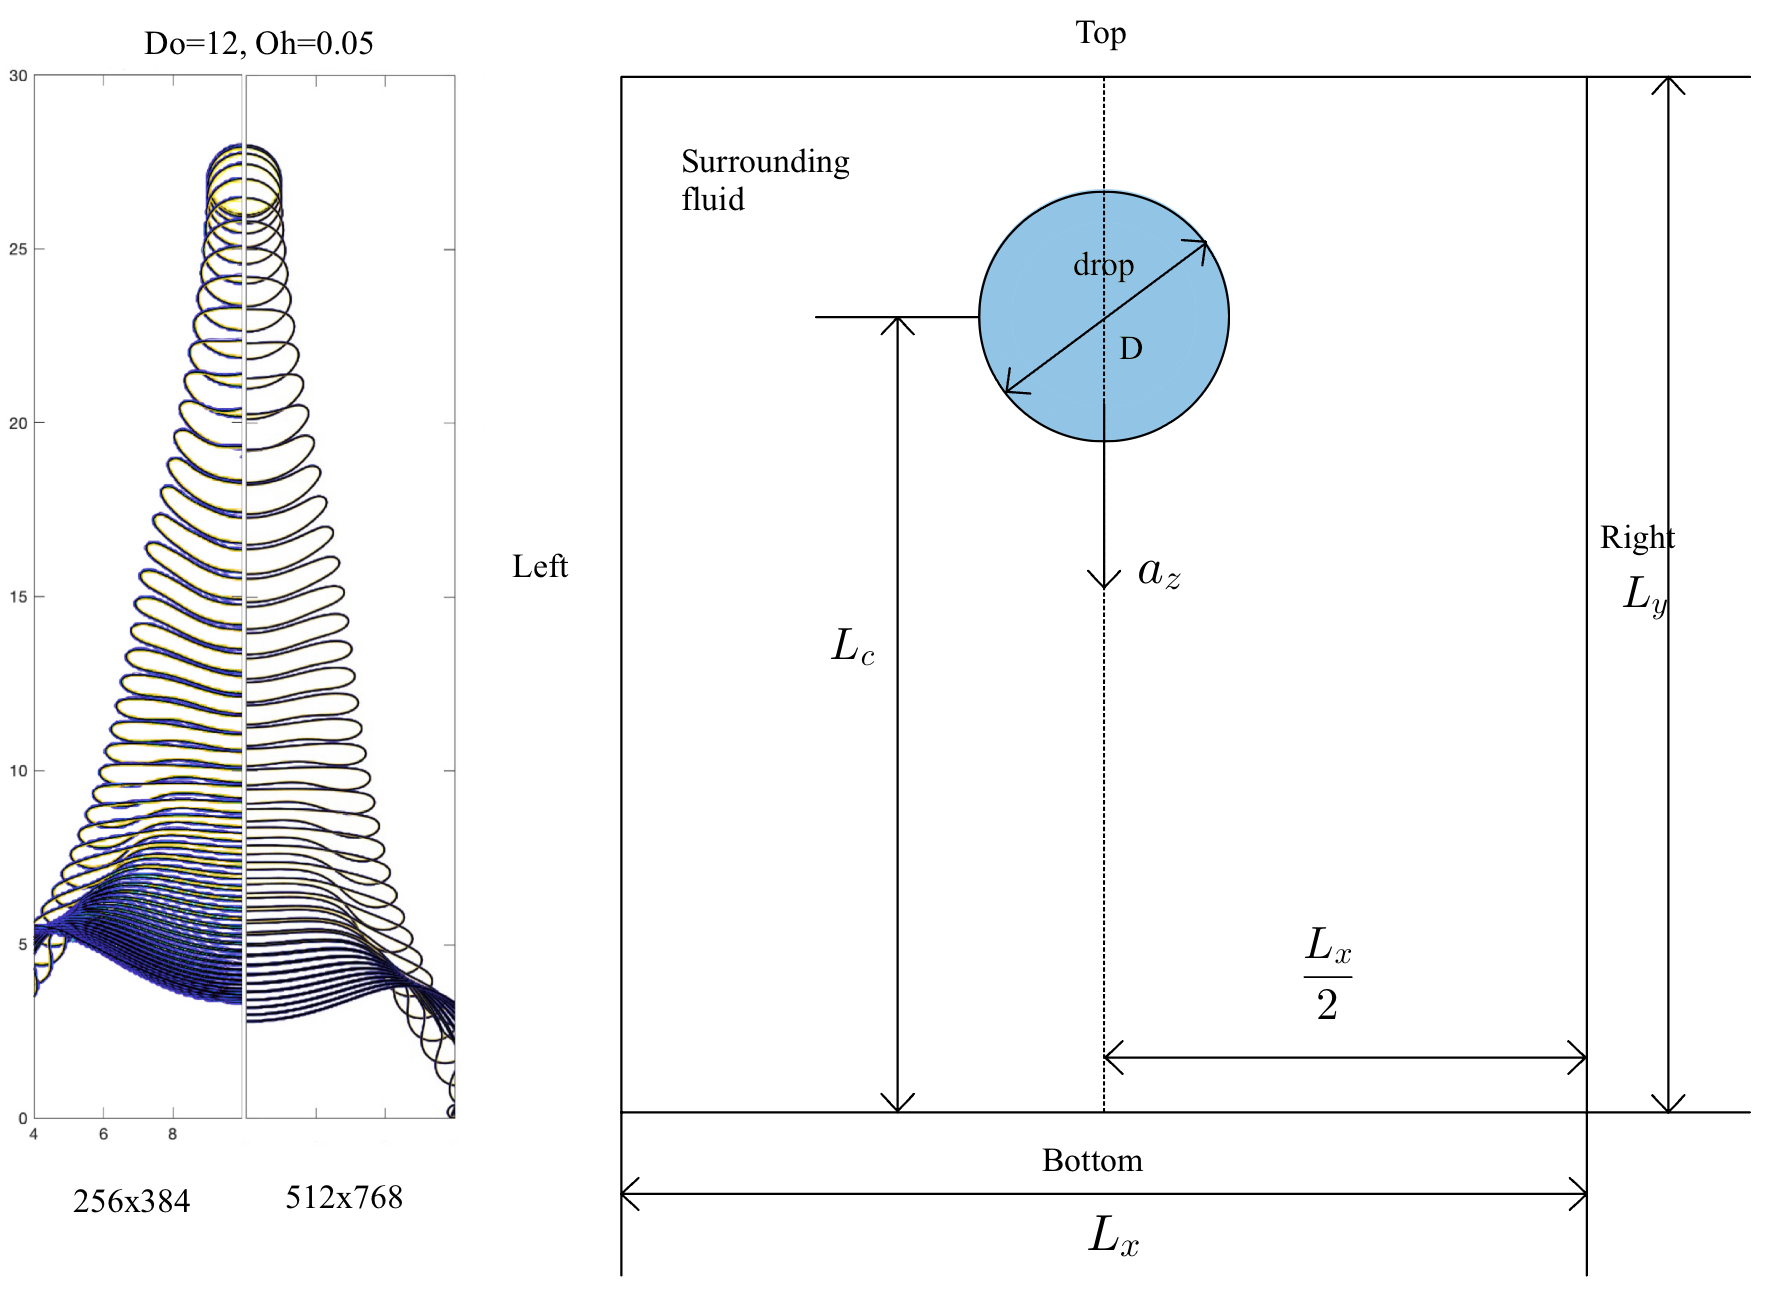
\includegraphics[width=0.8\textwidth]{Latex/figures/Domain_grid_indep.jpg}
    % \caption{Drop deformation as a function of the Reynolds number.}
    \label{deformation}
\end{figure}

In this part, we also performed the grid independence study to confirm the best resolution that could balance accuracy and cost, which includes time and computational resources. The finest grid resolution we could complete in time is 512x768, which actually costs 2 days on the computer to finish. After comparing with 256x384, we find that the 256x384 performs well, which means we can almost ignore the difference, and it can simulate and get results at high $Eo$.

\section{Results, Compare, and Discussion}

\subsection{Breakup Map}

\begin{figure}[H]
    \centering
    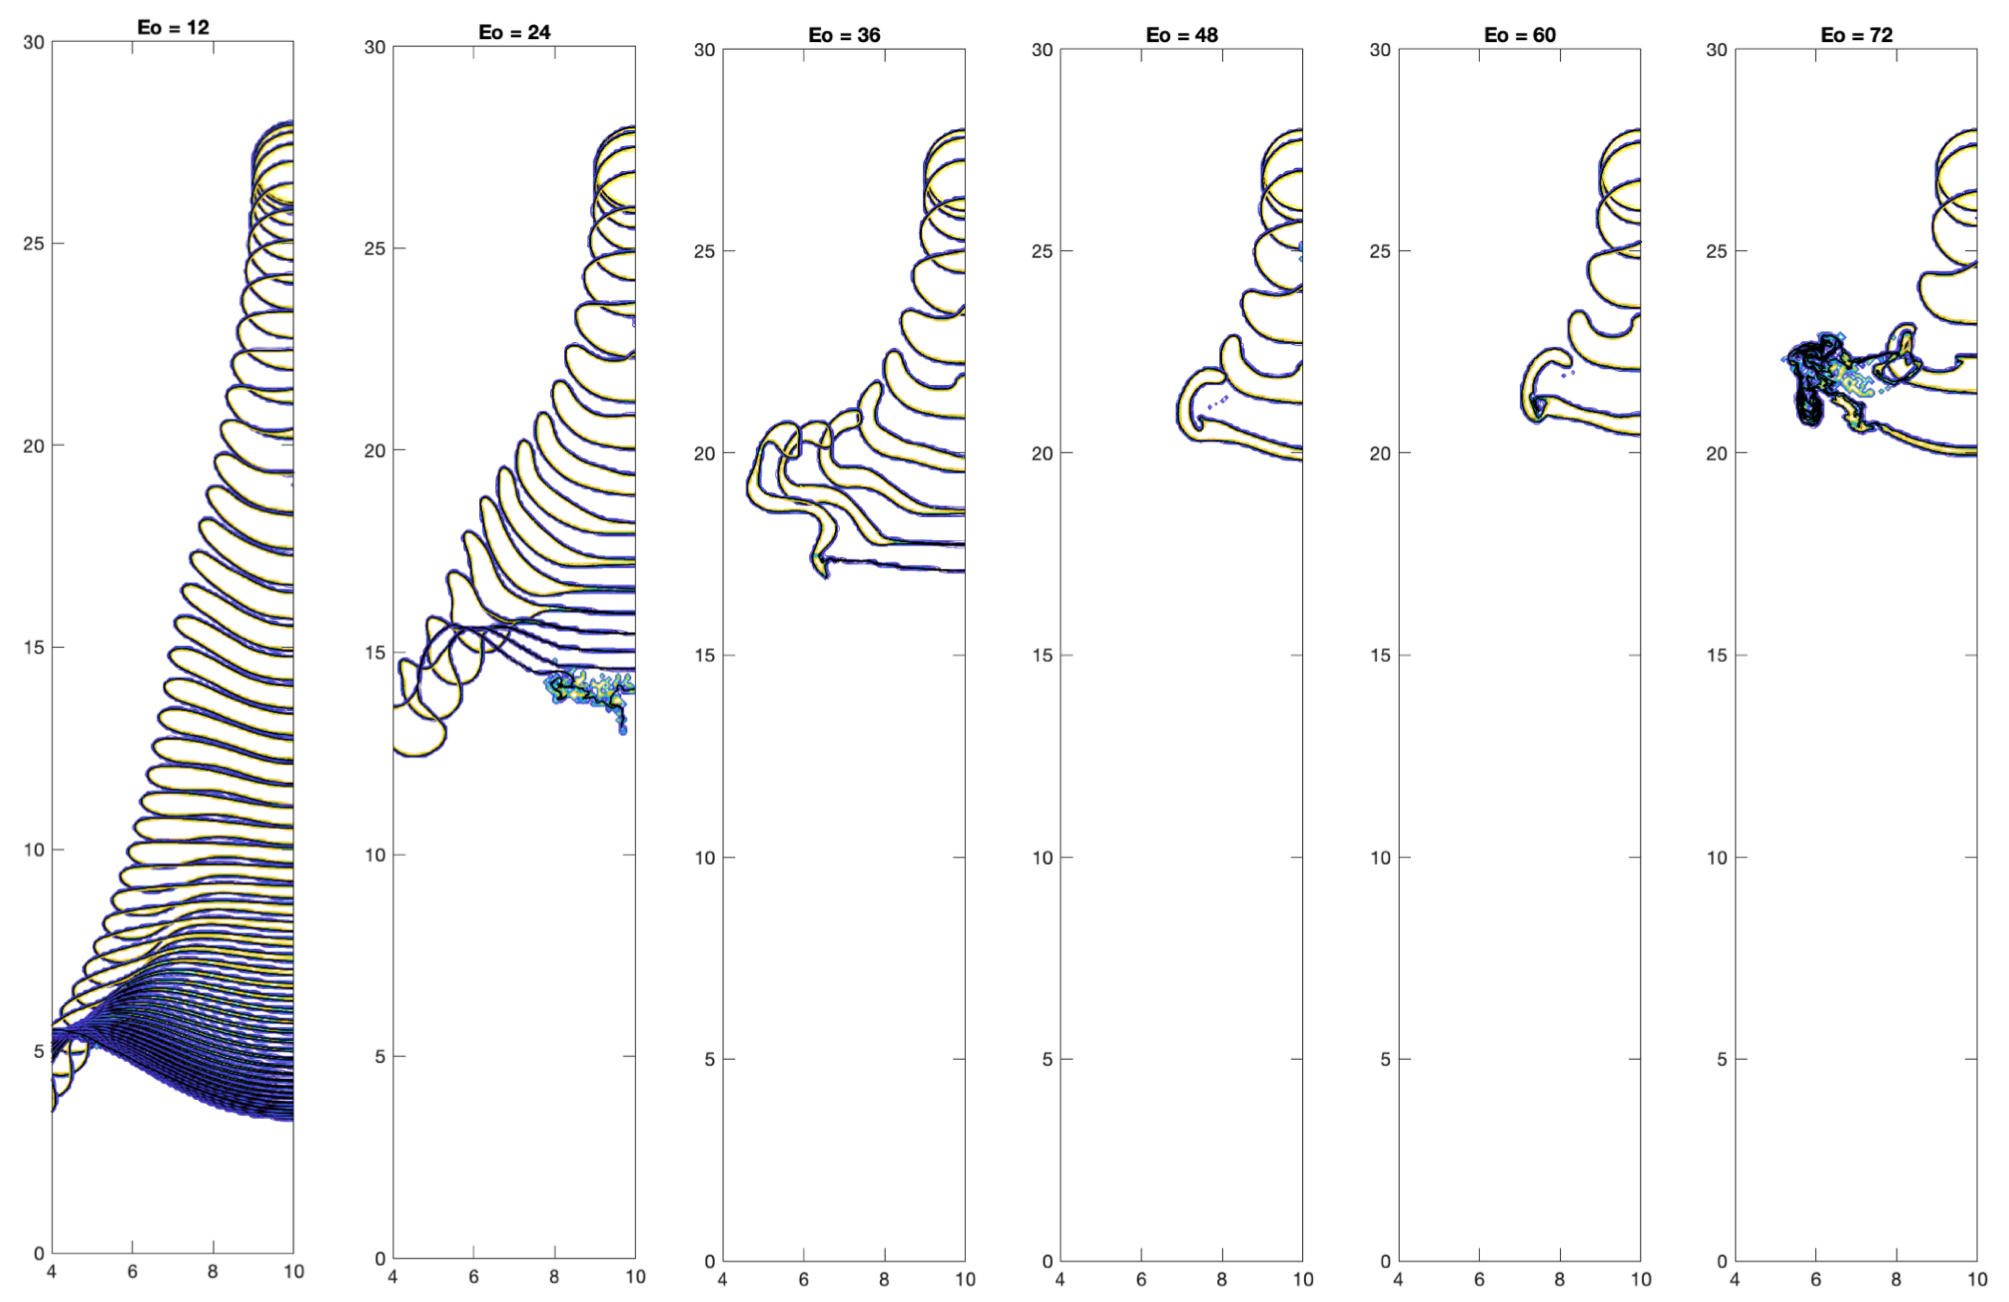
\includegraphics[width=0.6\textwidth]{figures/Eo_effect.jpg}
    \caption{Drop breakup map using different Eötvös number.}
    \label{fig:deformation}
\end{figure}

In the breakup map obtained for a 2D drop (or infinite cylinder in 3D), we observe the following trends:

\begin{itemize}
    \item Forward breakup (in the direction of the drop's motion) for $Eo = 12$ and $Eo = 24$.
    \item Backward breakup for $Eo > 24$, leading to a "disk-like" shape.
\end{itemize}

When $Eo$ is low (e.g., $Eo = 12$), gravitational forces dominate the motion of the falling drop. At this $Eo$ value, surface tension remains strong enough to maintain the drop's shape for a time, but it eventually leads to a slow breakup. Initially, the drop exhibits a near-spherical shape, but as it falls, the pressure at the front-center increases, pushing fluid toward the edges. This leads to elongation and flattening, eventually resulting in a backward-facing bag. As $Eo$ increases (e.g., $Eo = 24$), this process accelerates, and the edges flatten more rapidly, leading to the formation of a disk-like structure.

At higher $Eo$ values (e.g., $Eo = 48$ or above), surface tension is too weak to maintain the drop's shape. The drop initially forms a disk-like shape but soon retracts at the center, creating a narrow point between the edge and center. This thinning ultimately results in breakup, generating smaller droplets (shear breakup). These observations are consistent with experimental findings, though the exact breakup pattern may vary depending on the non-dimensional parameters.
\subsubsection{Compare to Axis-symmetric Simulation}



Compared to Dr. Han and Dr. Tryggvason's research results in 3D (axisymmetric), we found that in our 2D drop simulation (which can be modeled as an infinite cylinder), the evolution and breakup actually occurred at a smaller Eo number. This can be explained by the differences between the 2D and 3D schemes; however, the breakup patterns are quite similar.


\begin{figure}[H]
    \centering
    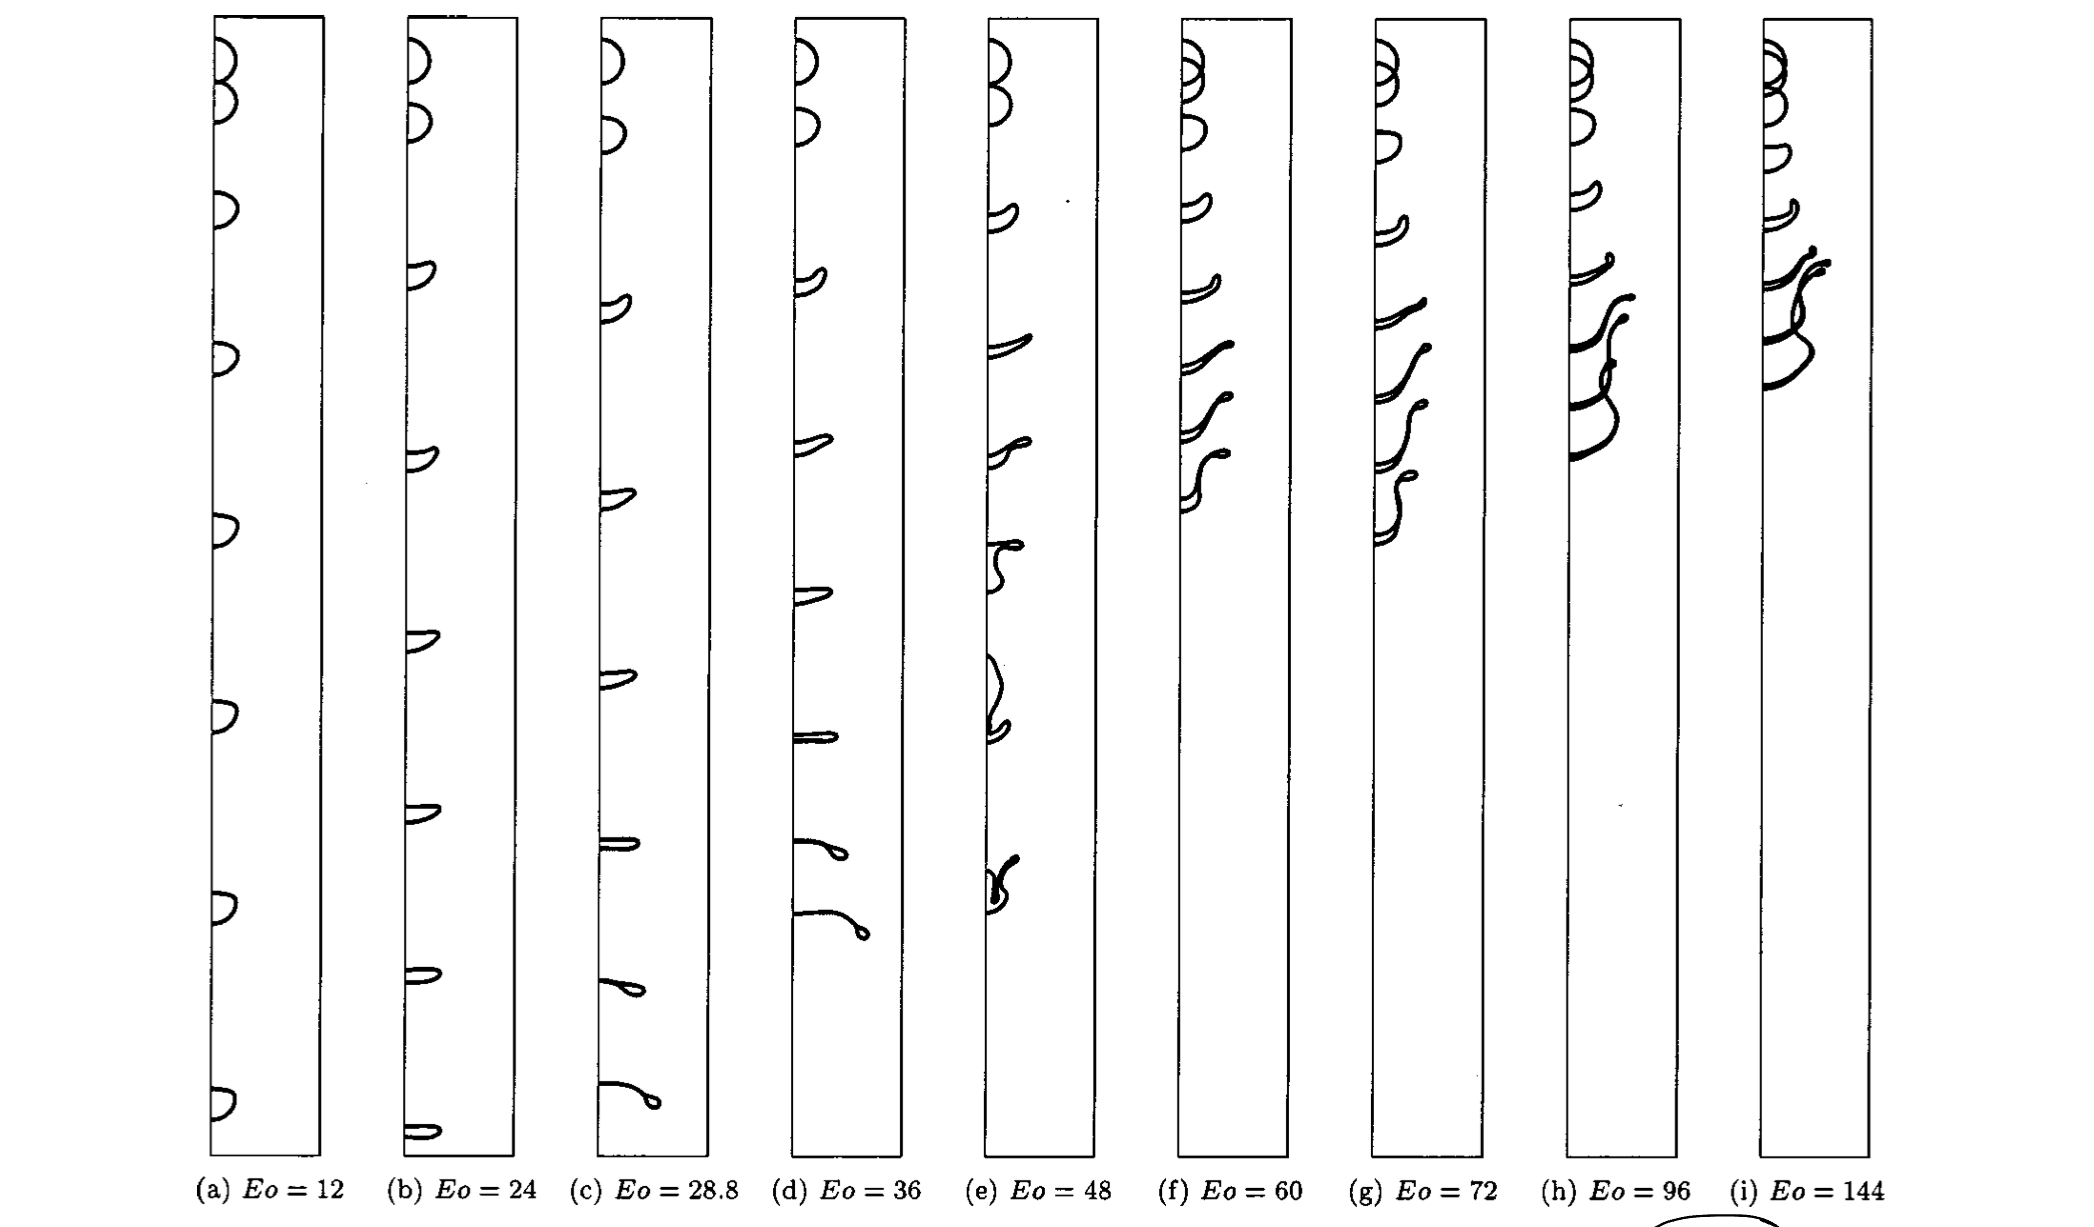
\includegraphics[width=0.6\textwidth]{Latex/figures/Trygg_allEo.jpg}
    \caption{Han and Tryggvason (1999) Axis-symmetric Breakup Map\cite{han1999axisymmetric}}
    \label{fig:deformation}
\end{figure}




\subsection{Center Velocity and Aspect Ratio}
Figure \ref{fig:velocity_aspect} shows the time evolution of the center velocity and aspect ratio for two different cases: (1) $Eo = 12$, $Oh = 0.05$, and (2) $Eo = 28.8$, $Oh = 0.125$, with a fixed density ratio $\rho_d / \rho_o = 10$.

\begin{figure}[H]
    \centering
    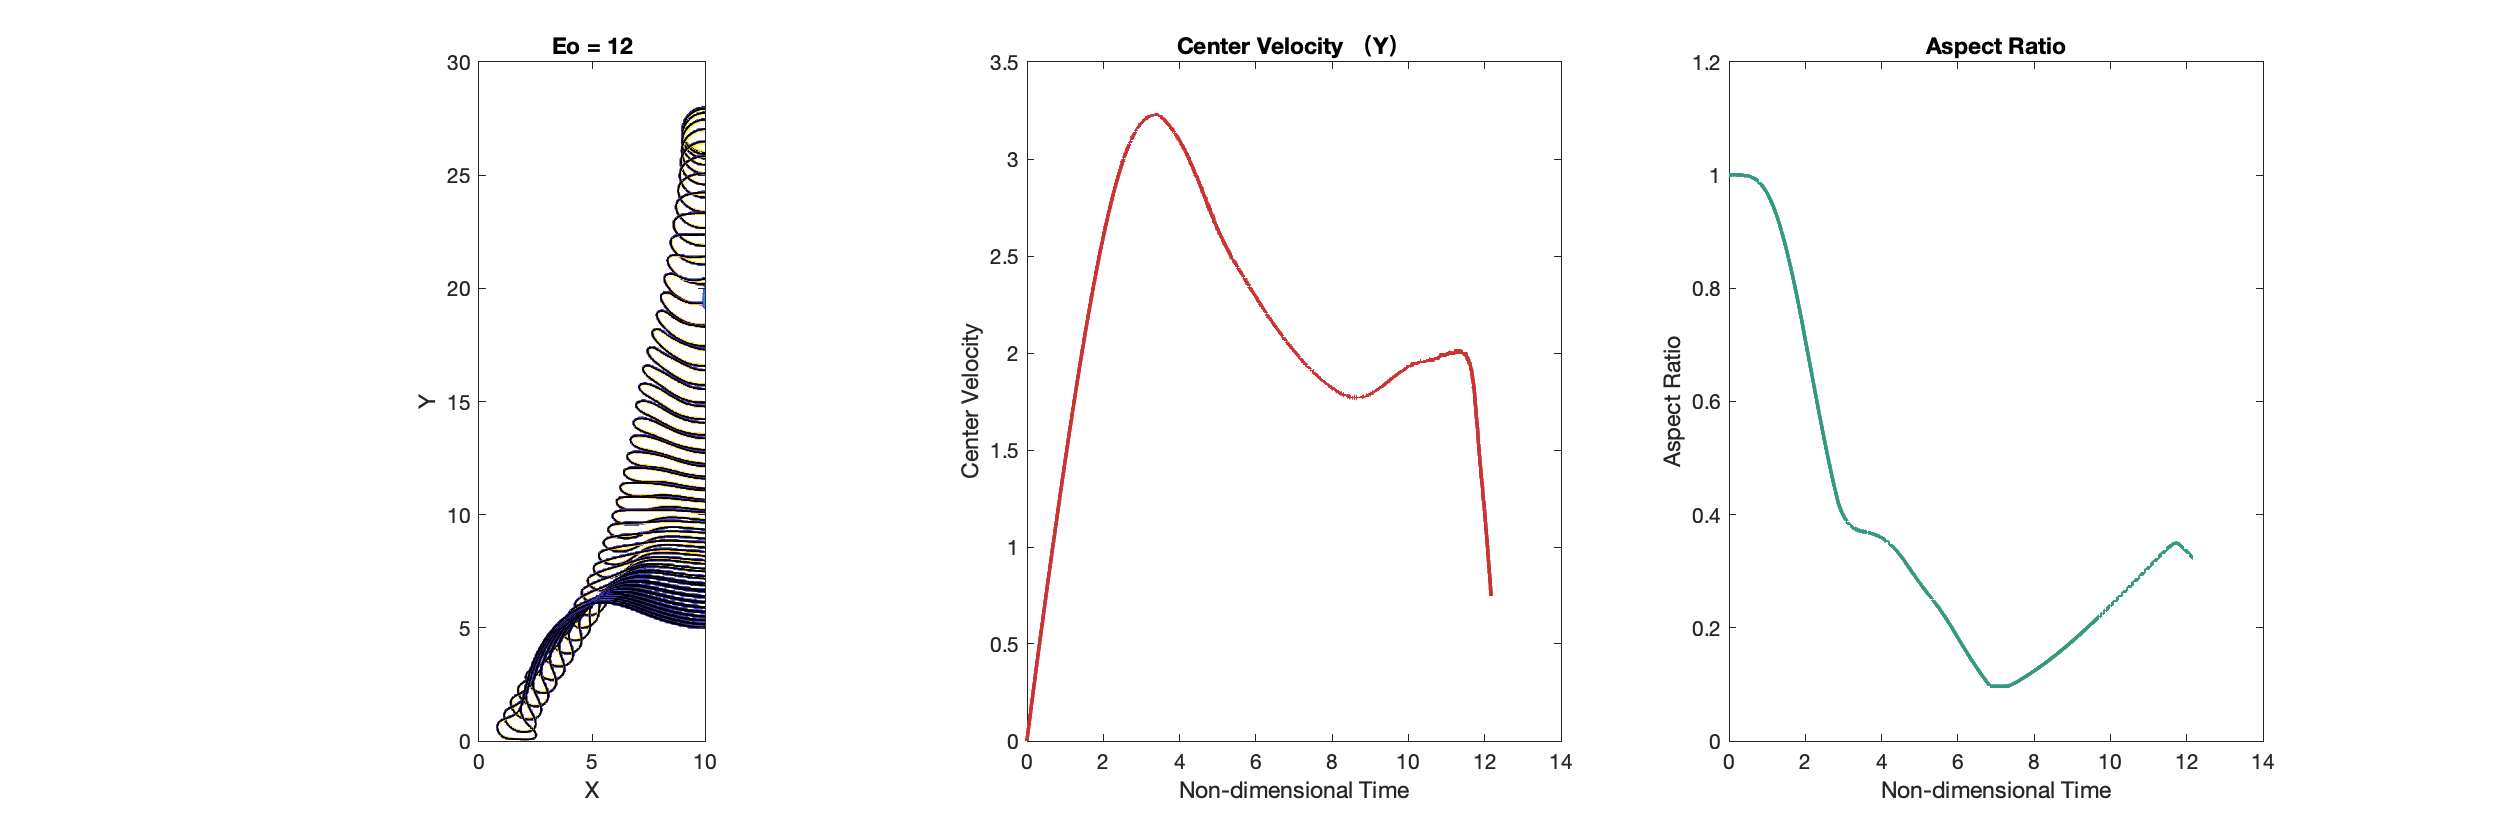
\includegraphics[width=\textwidth]{figures/All_Eo=12__t=0.28.png}
    \caption{Velocity and aspect ratio for $Eo = 12$, $Oh = 0.05$.}
    \label{fig:velocity_aspect}
\end{figure}

Initially, the drop's velocity increases due to gravity. As the drop deforms and drag forces build up, the velocity decreases. The aspect ratio exhibits minor changes at first but begins to drop as the edges flatten, reaching a minimum when the drop forms a bag-like structure.

\begin{figure}[H]
    \centering
    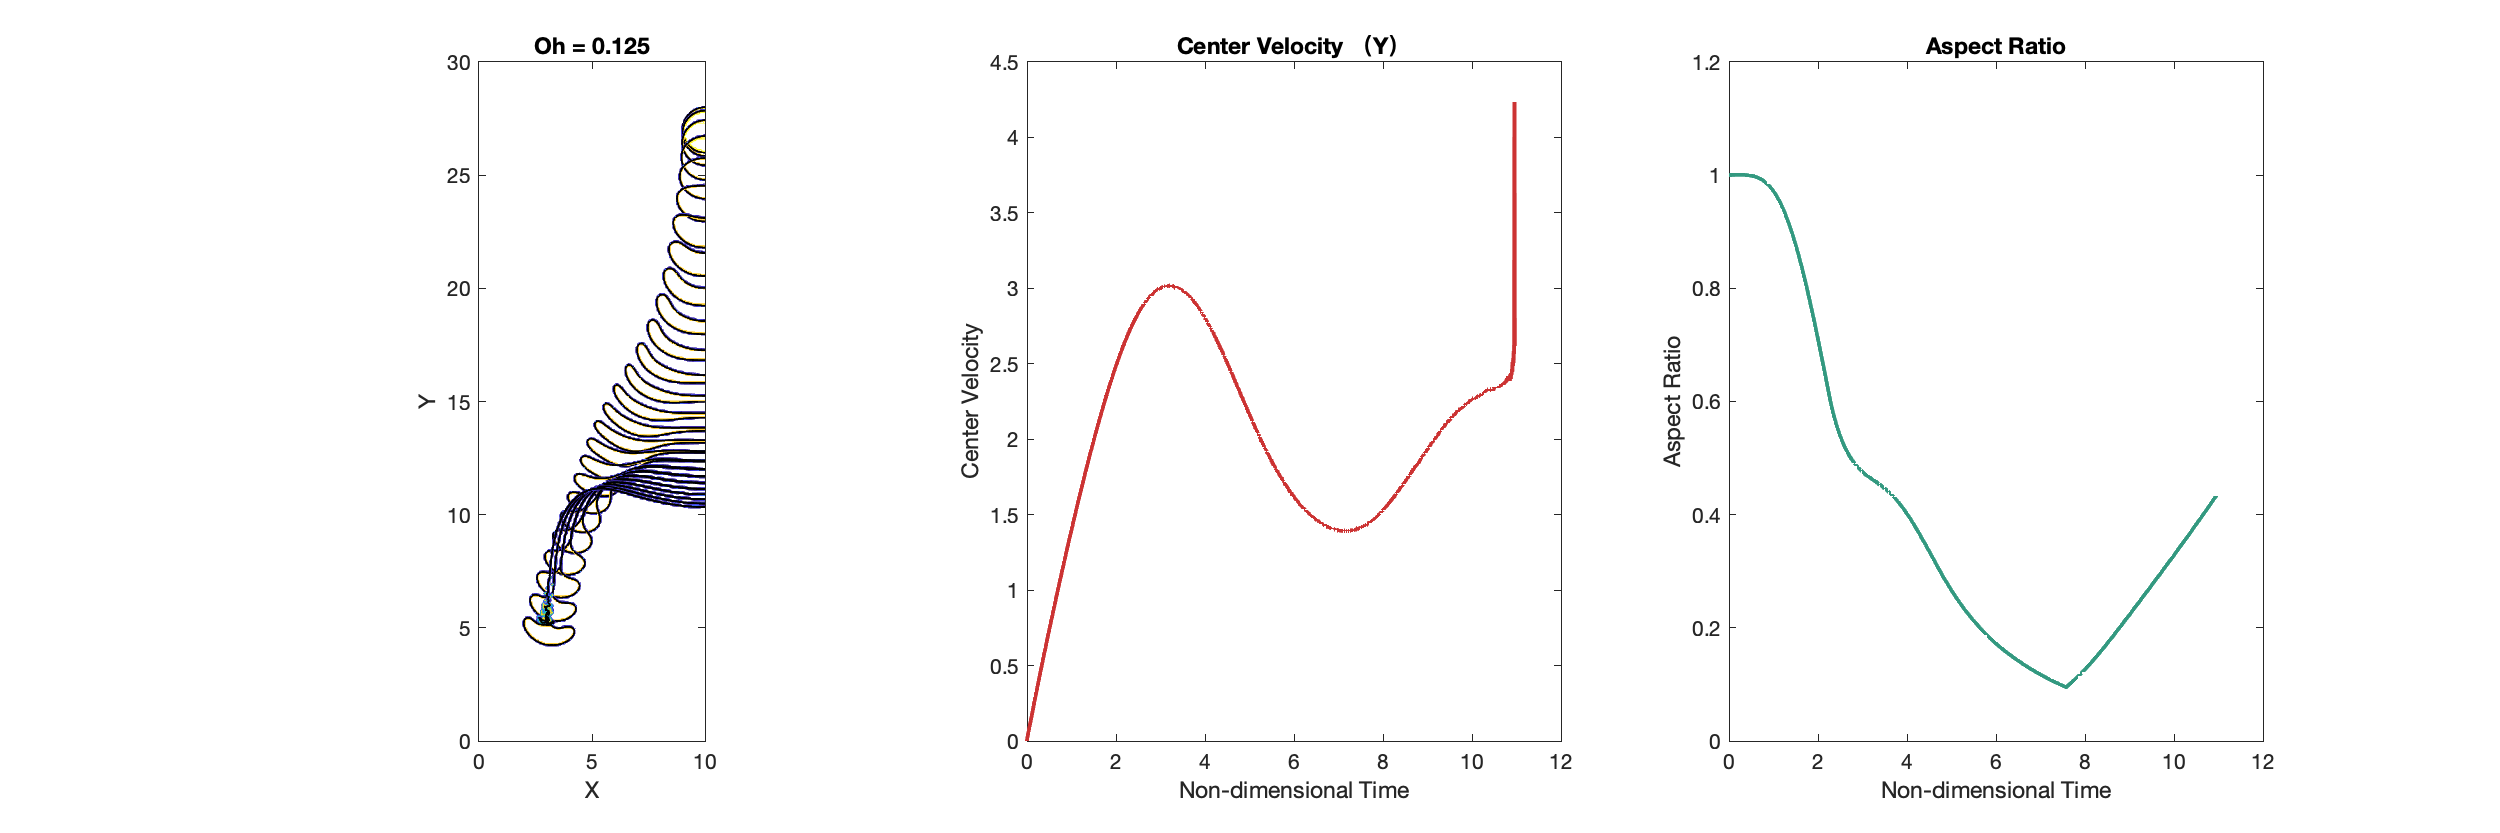
\includegraphics[width=\textwidth]{Latex/figures/All_Oh=1.25_t=0.44.png}
    \caption{Velocity and aspect ratio for $Eo = 28.8$, $Oh = 0.125$.}
    \label{fig:velocity_aspect}
\end{figure}

At the end of the simulation, we observe abnormal behavior in the velocity and aspect ratio curves. This is caused by the interaction between the drop's edge and the bottom boundary of the domain. As the drop's edge touches the boundary, velocity decreases sharply, and the aspect ratio calculation includes outer fluid, leading to an artificial increase. Future simulations could reduce these boundary effects by employing an extended domain or finer grid resolution near the boundaries.


\subsection{Center Velocity at Different $Eo$ Values}
Figure \ref{fig:velocity_comparison} compares the center velocity at different $Eo$ values ($Eo = 12$, $24$, $72$) to illustrate the effect of increasing Eötvös numbers on the drop’s motion. As $Eo$ increases, the drop's velocity decreases more rapidly, indicating that greater deformation and increased drag slow down the drop more significantly at higher $Eo$ values. For lower $Eo$ values (e.g., $Eo = 12$), the drop maintains its velocity for a longer period before experiencing significant deformation, resulting in a smoother decrease in velocity.

The comparison also highlights a key difference between 2D and 3D simulations. In 2D simulations like ours, the absence of an axis of symmetry results in lower drag, allowing the drop to move faster than in 3D cases. This explains why our velocity magnitudes are slightly higher than those reported in axisymmetric 3D simulations, such as those by Han and Tryggvason (1999). Nonetheless, the overall trends are consistent.

\begin{figure}[H]
    \centering
    \begin{minipage}{0.45\textwidth}
        \centering
        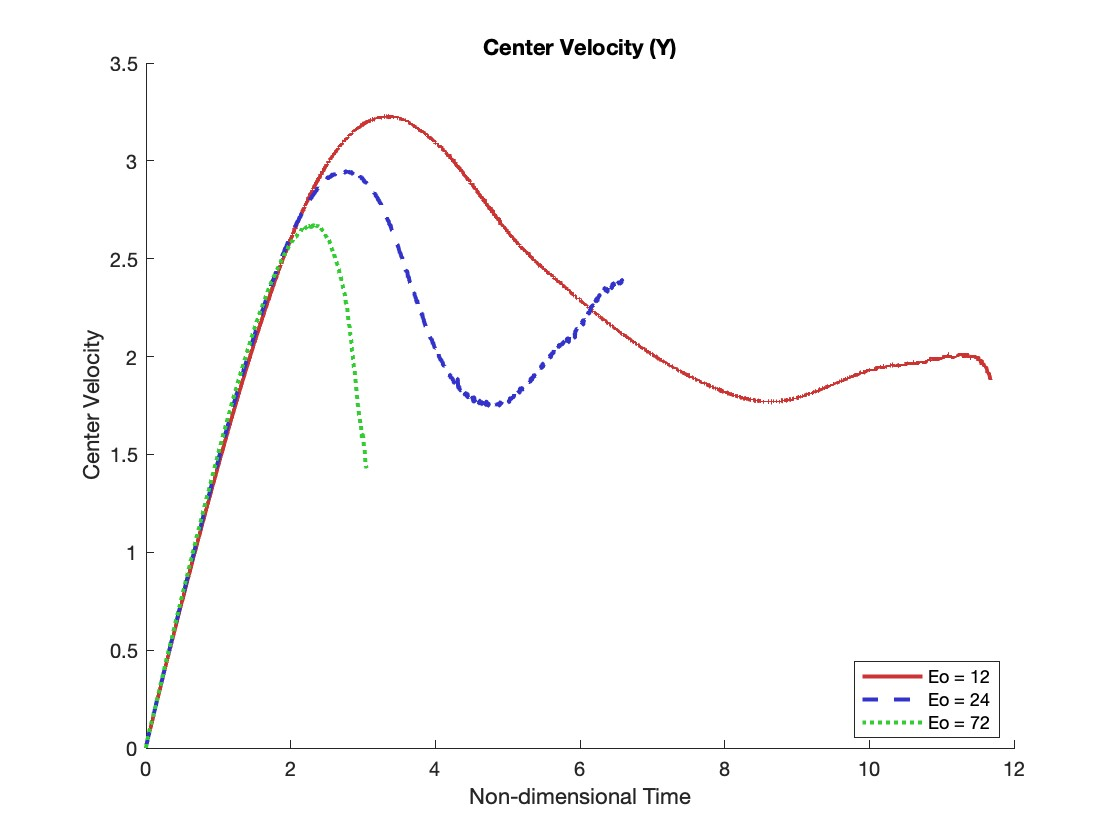
\includegraphics[width=\textwidth]{figures/velocity_profile_compare.jpg}
        \caption{Center velocity vs. time for $Eo = 12$, $24$, $72$.}
        \label{fig:velocity_comparison}
    \end{minipage}
    \hspace{0.05\textwidth}
    \begin{minipage}{0.45\textwidth}
        \centering
        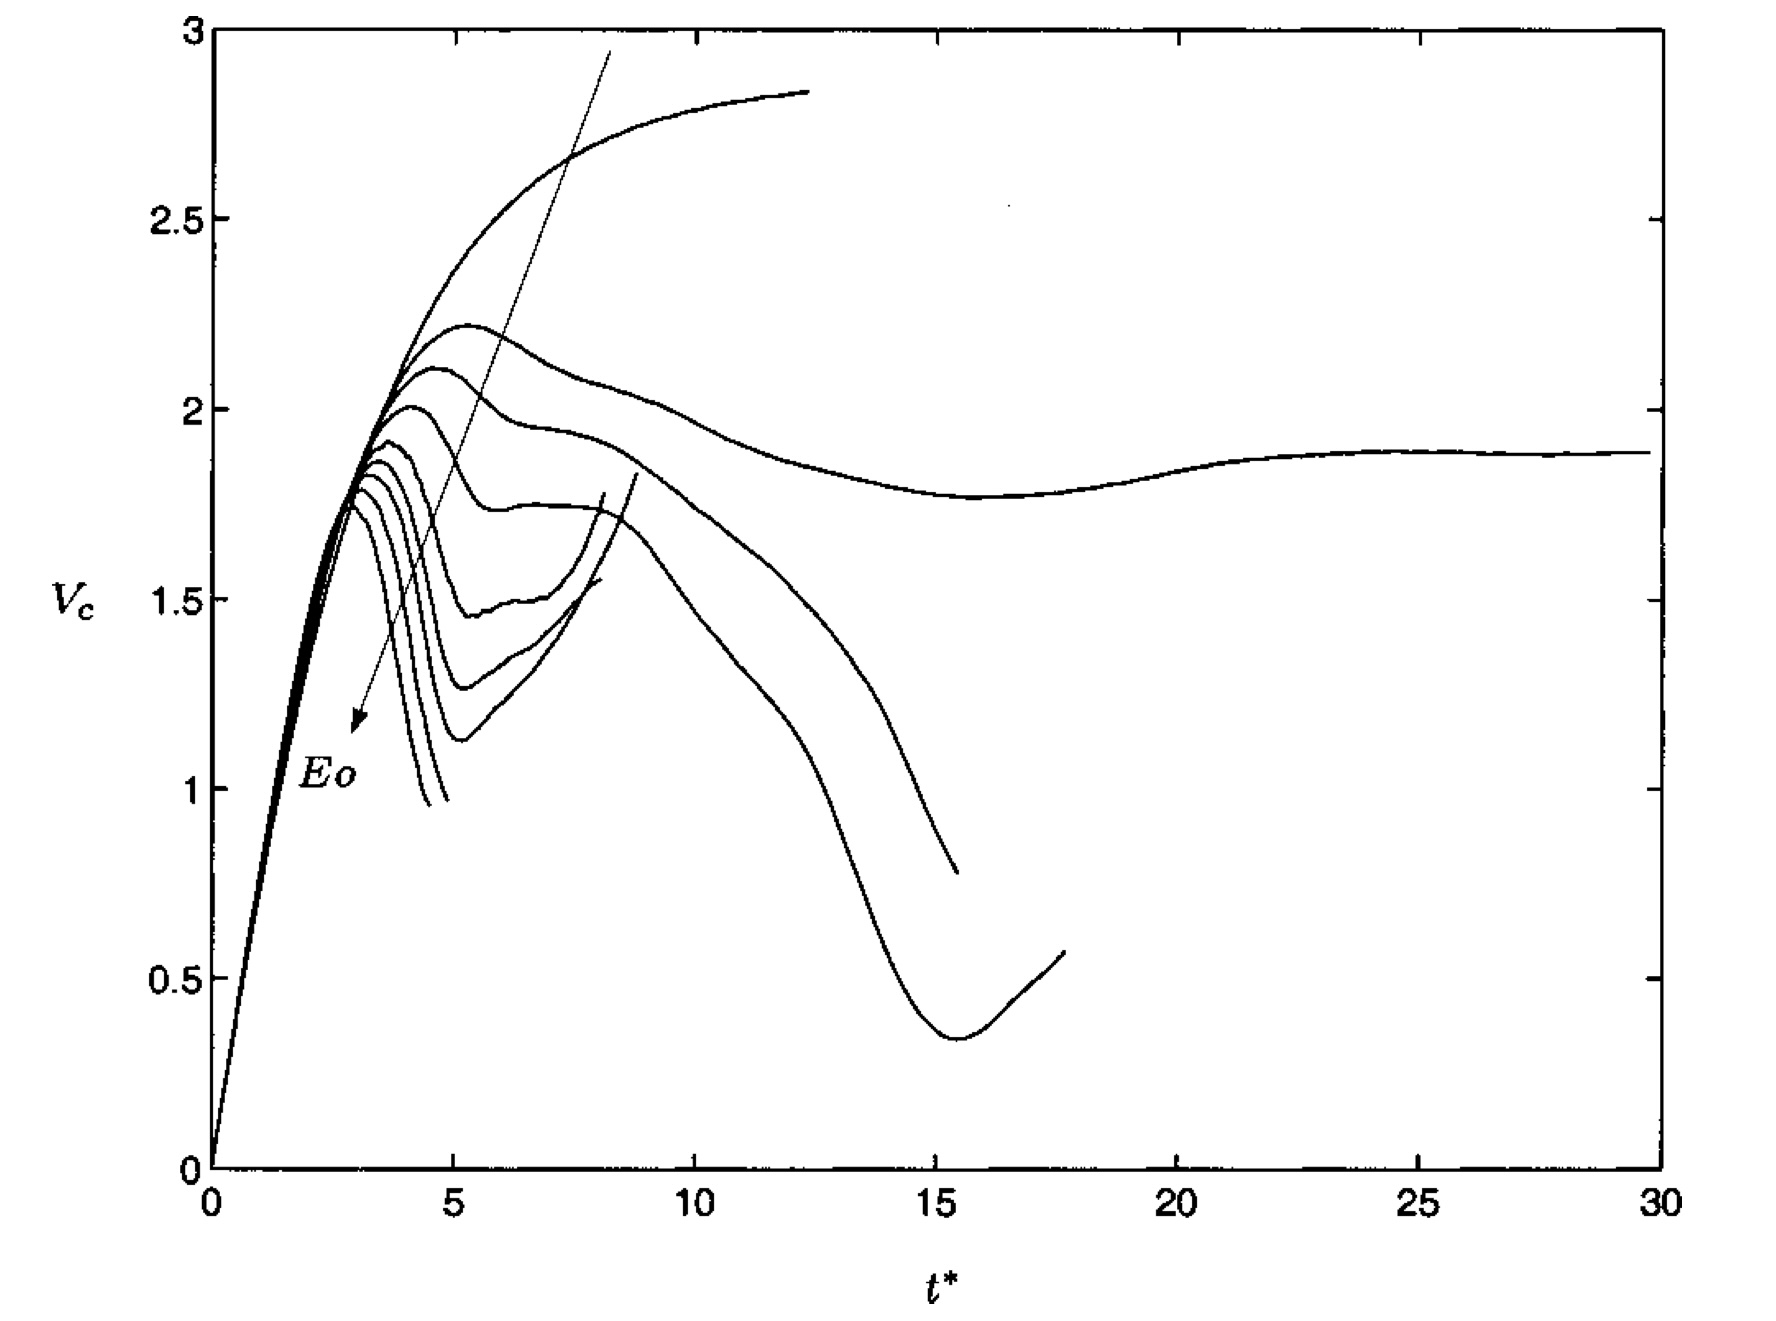
\includegraphics[width=\textwidth]{figures/Trygg_allEo_velo.jpeg}
        \caption{Han and Tryggvason (1999) velocity comparison for various $Eo$.}
        \label{fig:trygg_comparison}
    \end{minipage}
\end{figure}

Our results are qualitatively similar to those reported in Han and Tryggvason’s 3D simulations, showing that higher $Eo$ leads to faster deformation and more rapid velocity reduction. As the drop becomes more deformed, its drag increases, slowing down the drop at a much earlier stage than at lower $Eo$ values. While our simulations capture the essential physics of the problem, future work should aim to extend the model to 3D to further validate the results and achieve closer agreement with experimental data.


\bibliographystyle{plain}
\bibliography{references}

\end{document}
